\documentclass[../../../monografia.tex]{subfiles}
\graphicspath{ {images/}{../images/}{../../images/}{../../../images/} }

\begin{document}

\section{Test Setup}

As the main project is a simulation, the best way to validate the project was to create the same situation that was created in the simulation in real life. With that, it could compare the performance in the simulated environment with a similar real-life situation.

For it, we choose to use the Pioneer 2 DX \cite{pioneer2dx_2024}, the same robot that we used in the simulation, but as your simulation has not good support for communication protocols and PWM, we had to add one adapter between the information from the real robot and the bluepill.

In general, the Pioneer 2 DX adapter is responsible for getting all the information from the robot by communication protocol and sending it to the bluepill in the form of digital values with GPIOS. In contrast, the Pioneer 2 DX adapter is also responsible for getting velocity from each motor that the bluepill has sent and sending it back to pioneer 2DX.

It is possible to visualize the general schema in the figure \ref{fig: Test Setup - General}.

%---
\begin{figure}[h]
    \centering
    \caption{Test Setup - General}
    \centering % para centralizarmos a figura
    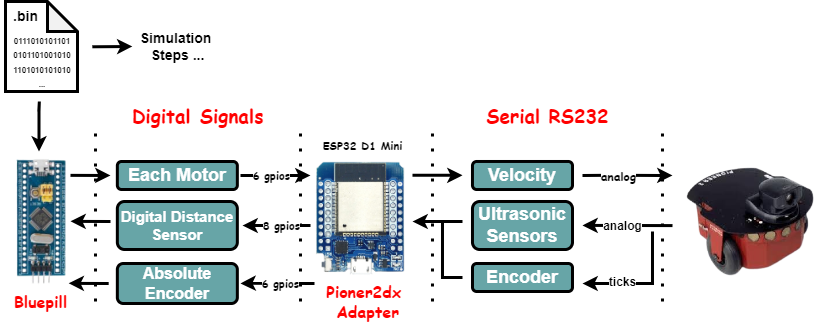
\includegraphics[width=16cm]{diagramas-test_setup-general.drawio.png}
    \label{fig: Test Setup - General}
\end{figure}
%---
\subsection{Hardware}

The hardware of the project has two main functionality:

\begin{itemize}
    \item {Connect the ESP32 D1 Mini with the bluepill}
    \item {Connect the ESP32 D1 Mini with the pioneer 2DX}
\end{itemize}

The connection between the Bluepill and the ESP32 is detailed in Table \ref{table: Connection between Esp32 and Bluepill}. A transistor is placed between the rst\_signal from the Bluepill and the ESP32 D1 Mini. This enables the ESP32 to be reset manually and ensures the signal stays high even when the Bluepill’s signal is low.

It is possible to check the whole developed pcb for this interface in our github repository in our organization \cite{pioneer_2dx_interface_pcb_2024}.

\begin{table}[h!]
\caption{Connection between Esp32 and Bluepill}
\begin{tabular}{|l|l|l|l|l|l|l|}
\cline{1-3} \cline{5-7}
Label       & Bluepill Pin & ESP32 Pin &  & Label         & Bluepill Pin & ESP32 Pin \\ \cline{1-3} \cline{5-7} 
DD1         & PA4          & SD3       &  & encoder1\_s1  & PB4          & CLK       \\ \cline{1-3} \cline{5-7} 
DD2         & PA5          & TCK       &  & encoder1\_s2  & PB3          & SD1       \\ \cline{1-3} \cline{5-7} 
DD3         & PA6          & IO5       &  & encoder1\_s3  & PB15         & IO2       \\ \cline{1-3} \cline{5-7} 
DD4         & PA7          & IO25      &  & encoder2\_s1  & PC13         & NC        \\ \cline{1-3} \cline{5-7} 
DD5         & PB0          & IO19      &  & encoder2\_s2  & PC14         & SD2       \\ \cline{1-3} \cline{5-7} 
DD6         & PB1          & IO18      &  & encoder2\_s3  & PC15         & CMD       \\ \cline{1-3} \cline{5-7} 
DD7         & PB10         & IO26      &  & motor1\_comm1 & PB7          & TDI       \\ \cline{1-3} \cline{5-7} 
DD8         & PB11         & SVP       &  & motor1\_comm2 & PB6          & IO4       \\ \cline{1-3} \cline{5-7} 
rst\_signal & PB13         & RST       &  & motor1\_comm3 & PB5          & IO0       \\ \cline{1-3} \cline{5-7} 
p2dx\_con   & PB12         & SD0       &  & motor2\_comm1 & PA1          & IO27      \\ \cline{1-3} \cline{5-7} 
            &              &           &  & motor2\_comm2 & PA2          & IO25      \\ \cline{1-3} \cline{5-7} 
            &              &           &  & motor2\_comm3 & PA3          & IO32      \\ \cline{1-3} \cline{5-7} 
\end{tabular}
\label{table: Connection between Esp32 and Bluepill}
\end{table}

To connect the ESP32 D1 Mini to the Pioneer 2DX, we used specific components for communication. The communication flow is illustrated in Figure \ref{fig: Test Setup - Hardware}, and the components' names and functions are detailed in Table \ref{table: Project main components}.

\begin{figure}
    \caption{Test Setup - Hardware}
    \centering
    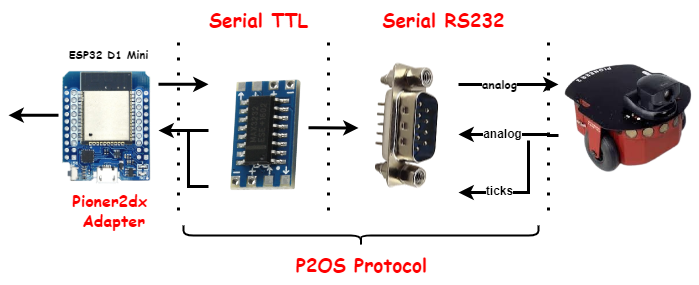
\includegraphics[width=16cm]{diagramas-test_setup-hardware.drawio.png}
    \label{fig: Test Setup - Hardware}
\end{figure}


\begin{table}[h!]
\caption{Project main components}
\begin{tabular}{@{}ll@{}}
\toprule
Main Component                                 & Function                                                              \\ \midrule
\multicolumn{1}{|l|}{Bluepill} &
  \multicolumn{1}{l|}{\begin{tabular}[c]{@{}l@{}}Main microcontroller of the project, it is resposible to receive\\  the same code that is received in the simulation\end{tabular}} \\ \midrule
\multicolumn{1}{|l|}{Esp32 D1 Mini} &
  \multicolumn{1}{l|}{\begin{tabular}[c]{@{}l@{}}Microcontroller used to create a interface between bluepill and \\ pioner 2 DX\end{tabular}} \\ \midrule
\multicolumn{1}{|l|}{Max3232}                  & \multicolumn{1}{l|}{Conversor between Serial TTL and Serial RS232}    \\ \midrule
\multicolumn{1}{|l|}{DB9 Connector}            & \multicolumn{1}{l|}{Connector type DB9, widely used for serial RS232} \\ \midrule
\multicolumn{1}{|l|}{2 LM317 Linear regulator} & \multicolumn{1}{l|}{Linear regulator for 3.3V and 5V}                 \\ \bottomrule
\end{tabular}
\label{table: Project main components}
\end{table}

It is also possible to visualize the whole connection in the figure \ref{fig: Test Setup - ESP32 Connections}. The whole schematic can be visualized in Appendix \ref{ap:Pioneer 2DX Interface Hardware}

\begin{figure}[h!]
    \caption{Test Setup - ESP32 Connections}
    \centering
    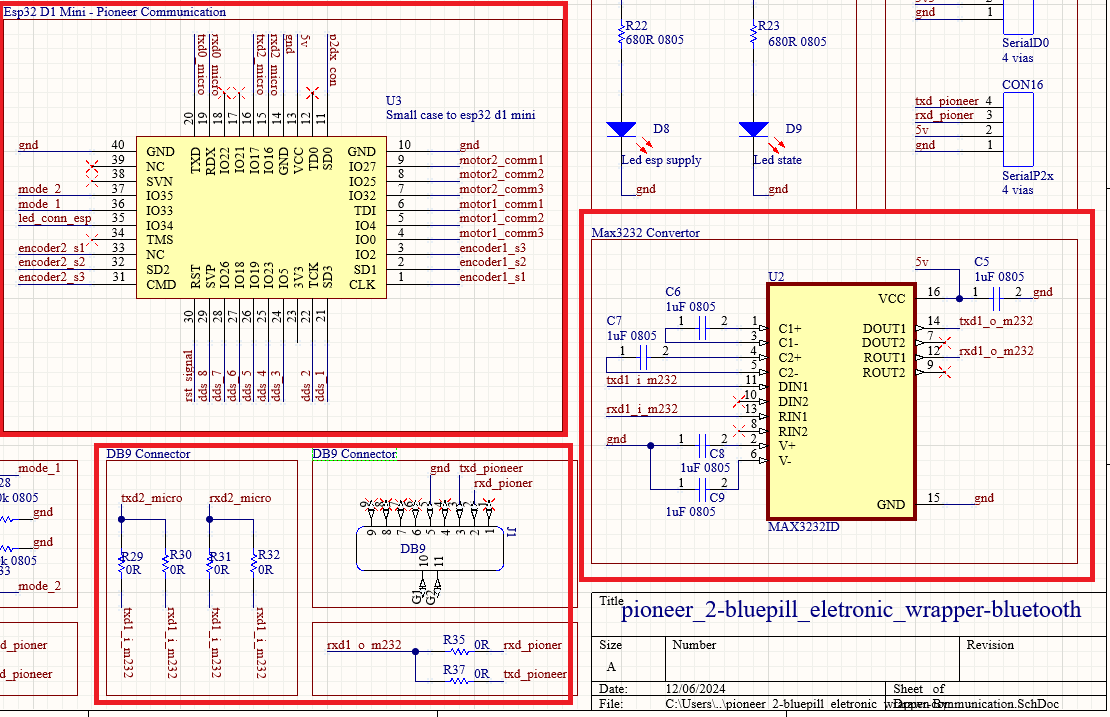
\includegraphics[width=16cm]{test_setup-hardware_connection.png}
    \label{fig: Test Setup - ESP32 Connections}
\end{figure}

\subsection{Pioneer 2DX Interface Firmware}

The Pioneer 2DX Interface has the mission to perform the computational logic behind the communication with the Pioneer 2DX and enable for an outside electronic device to send and receive data from the robot. Being more specific for this project, the Pioneer 2DX interface firmware has three main tasks:

\begin{itemize}
    \item {Connect the ESP32 D1 Mini with the bluepill}
    \item {Connect the ESP32 D1 Mini with a ps5 controller}
    \item {Connect the ESP32 D1 Mini with the pioneer 2DX}
\end{itemize}

The Pioneer 2DX interface allows either a PS5 controller or the Bluepill device to send data to the ESP32, but never simultaneously, as shown in Figure \ref{fig: Test Setup - Pioneer 2dx Interface}. The complete code developed for this interface is available in the GitHub repository of our organization \cite{pioneer_2dx_interface_esp32_2024}.

\begin{figure}[h!]
    \caption{Test Setup - Pioneer 2dx Interface}
    \centering
    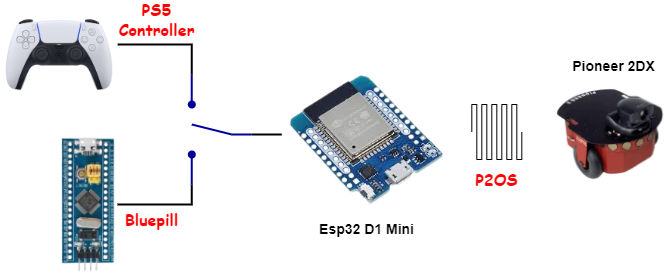
\includegraphics[width=16cm]{diagramas-test_setup-pioneer_2dx_interface.drawio.png}
    \label{fig: Test Setup - Pioneer 2dx Interface}
\end{figure}

\subsubsection{Bluepill Connection}

In general, the connection between the Bluepill and the ESP32 D1 Mini is performed through a digital signal. For example, the pins \textbf{motor2\_comm1}, \textbf{motor2\_comm2}, and \textbf{motor2\_comm3}. The pin \textbf{motor2\_comm3} represents the most significant bit, while \textbf{motor2\_comm1} represents the least significant bit. Check Figure \ref{fig: Test Setup - Encoder Data as Bits Example} to visualize an example for the encoder 1 data. It is also possible to check all the connection pins between the Bluepill and the ESP32 D1 Mini in Figure \ref{table: Connection between Esp32 and Bluepill}.

\begin{figure}[h!]
    \caption{Test Setup - Encoder Data as Bits Example}
    \centering
    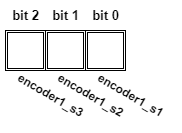
\includegraphics[width=6cm]{diagramas-test_setup-pioneer_2dx_interface-bluepill.drawio.png}
    \label{fig: Test Setup - Encoder Data as Bits Example}
\end{figure}


\begin{lstlisting}[language=C++, caption={BluepillCommunication::loop() function}]
int16_t linear_vel = (
    (this->motor\_gpio\_state[0] << 2)
    | (this->motor_gpio_state[1] << 1)
    | (this->motor_gpio_state[2])
);

int16_t angular_vel = (
    (this->motor_gpio_state[3] << 2) 
    | (this->motor_gpio_state[4] << 1) 
    | this->motor_gpio_state[5]
);
\end{lstlisting}

\subsubsection{Ps5 Controller Connection}

\subsubsection{Pioner 2DX communication}

\subsection{Bluepill test Firmware}


\end{document}

\begin{table}[h!]
\centering
\begin{tabular}{|c|c|c|}
\hline
\textbf{Pin Number} & \textbf{Esp32 Pin name} & \textbf{Label} \\ \hline
40 & GND  & gnd \\ \hline
39 & NC   & X \\ \hline
38 & SVN  & X \\ \hline
37 & IO35 & mode\_2 \\ \hline
36 & IO33 & mode\_1 \\ \hline
35 & IO34 & led\_conn\_esp \\ \hline
34 & TMS  & X \\ \hline
33 & NC   & encoder2\_s1 \\ \hline
32 & SD2  & encoder2\_s2 \\ \hline
31 & CMD  & encoder2\_s3 \\ \hline
30 & RST  & rst signal \\ \hline
29 & SVP  & dds\_8 \\ \hline
28 & IO26 & dds\_7 \\ \hline
27 & IO18 & dds\_6 \\ \hline
26 & IO19 & dds\_5 \\ \hline
25 & IO23 & dds\_4 \\ \hline
24 & IO5  & dds\_3 \\ \hline
23 & 3V3  & X \\ \hline
22 & TCK  & dds\_2 \\ \hline
21 & SD3  & dds\_1 \\ \hline
20 & TXD  & txd0\_micro \\ \hline
19 & RDX  & rxd0\_micro \\ \hline
18 & IO22 & X \\ \hline
17 & IO21 & X \\ \hline
16 & IO17 & txd2\_micro \\ \hline
15 & IO16 & rxd2\_micro \\ \hline
14 & GND  & gnd \\ \hline
13 & VCC  & 5v \\ \hline
12 & TD0  & X \\ \hline
11 & SD0  & p2dx\_con \\ \hline
10 & GND  & gnd \\ \hline
09 & IO27 & motor2\_comm1 \\ \hline
08 & IO25 & motor2\_comm2 \\ \hline
07 & IO32 & motor2\_comm3 \\ \hline
06 & TDI  & motor1\_comm1 \\ \hline
05 & IO4  & motor1\_comm2 \\ \hline
04 & IO0  & motor1\_comm3 \\ \hline
03 & IO2  & encoder1\_s3 \\ \hline
02 & SD1  & encoder1\_s2 \\ \hline
01 & CLK  & encoder1\_s1 \\ \hline
\end{tabular}
\caption{ESP32 Pin Mapping for Pioneer Communication}
\end{table}